\section{Problemstellung}
Wie in der Einleitung bereits angemerkt, beschreibt \glqq Information Retrieval\grqq das Bereitstellen spezieller Informationen aus einer meist großen, unsortierten Datenmenge. Dabei bekommt das System eine vom Nutzer gestellte Query (Abfrage) und versucht auf dessen Basis, Daten, die meist als Dokumente vorliegen, zurückzuliefern.
Im Gegensatz zu Abfragen im Datenbankumfeld beinhaltet die Query jedoch keinerlei Informationen, um ein spezielles Element eindeutig identifizieren zu können. Dies soll ein IR-System auch nicht leisten. Vielmehr sollen Ergebnisse zurückgeliefert werden, die mit hoher Wahrscheinlichkeit Relevanz bzgl. der gestellten Query besitzen. Der Nutzer selektiert dann die für diesen nötigen Dokumente.
\newline
Mathematisch lässt sich dies folgendermaßen formulieren:
Aus einer Dokumentenmenge $D$ soll mithilfe einer Funktion eine Teilmenge $D_1$ von $D$ ermittelt werden, die relevant für eine Abfrage $q$ ist.
\newline
Um diese Funktion sinnvoll definieren zu können, muss jedoch zuvor die Menge aller Queries, sowie die Menge aller Tokens definiert werden:
\begin{defi}
	Sei $d \in D$ ein Dokument. Die Menge $T_d$ ist nun die Menge aller Wörter, die in dem Dokument $d$ enthalten sind: $T_d$ = $\{$$t_1$, .., $t_n$$\}$.
	\newline
	Die Menge $T$ ist die Menge aller Terme, die in den Dokumenten aus $D$ vorkommen, also:
	$T$ = $T_{d1} \cup .. \cup T_{dn}$ mit $d_i \in D$.
\end{defi}

\begin{defi}
	Mithilfe der letzten Definition kann nun die Menge aller möglichen Queries definiert werden:
	$Q \subseteq 2^T$
\end{defi}

\begin{defi}
	Eine Funktion $f$: $Q \rightarrow D_1$ heißt Retrievalfunktion, wobei $D_1 \subseteq D$ gilt und $Q$ die Menge aller Queries ist.
\end{defi}

Nachdem die Problemstellung formuliert ist, muss eine Strategie entwickelt werden, wie die Funktion $f$ dargestellt bzw. umgesetzt werden kann.

\newpage

\section{Strategiefindung}
Dieser Abschnitt soll eine Übersicht bieten, wie das im Folgenden vorgestellte IR-System arbeiten soll.
\newline
Als Vorarbeit müssen alle Dokumente, die im Index aufgenommen werden sollen, in eine Codierung wie ASCII oder Unicode umgewandelt werden. Dazu wird ein Tool genutzt, das hier nicht weiter von Relevanz sein wird.
Es sollen mindestens all diejenigen Dokumente in den Index aufgenommen werden, die im PDF-Format vorliegen.
\newline
Der erste Schritt, der das IR-System an sich leisten muss, ist das Erstellen von Tokens. Dazu wird jedes Dokument in Tokens aufgespalten. Ein Token ist in den meisten Fällen ein Wort, Satzzeichen wie Leerzeichen, Kommata usw. sollen nicht als Tokens behandelt werden und werden ignoriert.
\newline
Für jeden Token wird es später im Index einen Eintrag geben, der eine Liste mit weiteren Informationen hält. Diese Liste muss mindestens die Dokument-ID speichern, in dem das Token steht. In diesen Listen werden häufig noch weitere Informationen hinterlegt, beispielsweise die Häufigkeit eines Tokens.
\newline
Der zweite große Schritt besteht darin, einen Algorithmus zu entwerfen, der eine Query entgegennimmt und auf Basis der Query und des Index eine Liste von relevanten Dokumenten ausgibt. Dieser wird das in der Einleitung kurz vorgestellte Vektorraummodell verwenden. Weiter wird dieser für die Ermittlung der Relevanz die sogenannte TF-IDF-Gewichtung nutzen. Diese wird später noch ausführlich vorgestellt.
\newline
Neben diesen beiden Punkten wird der Index komprimiert, um Speicherplatz zu sparen und die Performance zu erhöhen.

\section{Tokenization}
\subsection{Vorarbeiten}
Bevor aus Dokumenten Tokens erzeugt werden können, müssen einige Fragen beantwortet werden.
Eine Frage ist, welche Dokumente betrachtet werden sollen und wie man ein Dokument definiert. Zur Veranschaulichung dieses Problems, soll ein Beispiel dienen:
\newline
Angenommen das IR-System soll dazu dienen Dokumente auf der Festplatte eines Computers zu finden. In diesem Szenario kann jede in einem Ordner gelistet Datei als Dokument angesehen werden. Dies wäre der einfachste Fall. Jedoch ist dies meist nicht erwünscht. So sollen beispielsweise bestimmte Dateitypen von der Suche ausgeschlossen werden. In UNIX existiert ein Dateityp, welcher Mails speichert. Hier soll jede Mail als einzelnes Dokument angesehen werden, die Datei muss also in mehrere Dokumente aufgespalten werden \cite{IR_Intro_Cambridge}.
Umgekehrt gibt es Szenarien, in denen mehrere Dokumente zu einem Dokument zusammengefasst werden müssen, um bei der Suche nutzbare Ergebnisse zu erzielen \cite{IR_Intro_Cambridge}.
\newline
Ein weiteres Problem, das gelöst werden muss, um die Dokumente verarbeiten zu können, ist die Codierung der Inhalte der Dokumente. Hierbei müssen Dokumente, die meist in vielen unterschiedlichen Codierungen vorliegen, zu einer definierten Codierung überführt werden \cite{IR_Intro_Cambridge}.
\newline
Diese Probleme der \glqq Vorarbeit\grqq werden in der später gezeigten Beispielimplementierung nicht behandelt, sondern von anderen Tools behandelt.

\subsection{Tokenerzeugung}
Sobald definiert ist, was als Dokument verstanden wird (engl. document unit) und ist eine einheitliche Codierung der Dokumente vereinbart, können die Dokumente in Tokens aufgeteilt werden.
\newline
Zunächst jedoch drei wichtige Definitionen:
\begin{defi}
	Unter einem Token wird eine zusammenhängende Zeichenkette verstanden, die innerhalb eines Dokuments vorkommt \cite{IR_Intro_Cambridge}.
\end{defi}
\begin{defi}
	Ein Typ bezeichnet eine Klasse von Tokens, die dieselben Zeichen enthalten \cite{IR_Intro_Cambridge}.
\end{defi}
\begin{defi}
	Ein Term ist ein Typ, welcher im Dictionary eines IR-System vorkommt \cite{IR_Intro_Cambridge}.
\end{defi}

Eine wichtige Frage, die im Rahmen der Tokenerzeugung geklärt werden muss, ist, welche Zeichenketten als Token behandelt werden. Kommata, Punkte und sonstige Satzzeichen haben keine sinnvolle Bedeutung im Zusammenhang mit Information Retrieval, diese Zeichen können somit aus Tokens entfernt bzw. während der Tokenerzeugung überlesen werden \cite{IR_Intro_Cambridge}.

Der Text
\begin{center}
	\textit{Beispielsatz, der ein Komma hat.}
\end{center}
erzeugt diese Tokenmenge:
\begin{center}
	$Tokens$ = $\{$\textit{Beispielsatz}, \textit{der}, \textit{ein}, \textit{Komma}, \textit{hat}$\}$
\end{center}

Einige Information Retrieval-System nutzen darüber hinaus sogenannte \glqq stop words\grqq. Das sind Wörter, die in sehr vielen Dokumenten in großer Anzahl vorkommen und damit wenig Bedeutung für die Suche besitzen \cite{IR_Intro_Cambridge}. Beispiele für solche Wörter sind \glqq ist\grqq, \glqq sein\grqq und \glqq und\grqq. Jedoch funktioniert diese Technik später beim Suchen schlechter als zunächst angenommen. Das Wort \glqq sein\grqq kann beispielsweise als Verb oder als Pronomen in einem Dokument vorkommen. Als Pronomen kann dieses Wort durchaus wichtig sein für eine Suche (beispielsweise innerhalb eines Buchtitels), wird jedoch als stop word aussortiert. Daher werden in neuen IR-Systemen entweder gar keine stop words oder nur eine geringe Anzahl stop words genutzt.
\newline
Eine weitere Möglichkeit solche Wörter zu filtern ist Stemming.
Diese Methode führt Wörter auf ihren Wortstamm zurück \cite{IR_Intro_Cambridge} \cite{IR_Uni_Bamberg}. Dadurch wird die Anzahl der Terme, die im Index gespeichert werden müssen, stark gesenkt. Allerdings bringt diese Methode eine Unschärfe mit sich. Damit ist gemeint, dass zwei nicht verwandte Wörter auf denselben Wortstamm zurückgeführt werden, wodurch bei der späteren Suche nach einem der beiden Urpsrungswörter auch Ergebnisse zurückgeliefert werden, die irrelevant für die Query sind \cite{IR_Intro_Cambridge}.
\newpage
Weiter existieren sprachspezifische Probleme. Beispielsweise wird im Englischen häufig mit Kurzformen von Wörtern gearbeitet, so wird \glqq are not\grqq zu \glqq aren't\grqq. Es muss geklärt werden wie mit solchen Formen umgegangen werden soll. Ein Ansatz ist Query Preprocessing. Hierbei werden Wörter dieser Art, die in der Query stehen, wie während der Tokenerzeugung in eine einheitliche Form gebracht \cite{IR_Intro_Cambridge}. Darüber hinaus gilt es zu beachten, dass Eigennamen wie \glqq Hewlett-Packard\grqq nicht oder nur nach bestimmten Regeln prozessiert werden dürfen. Welche Wörter als Eigenname behandelt werden und welche nicht, kann mittels Machine Learning-Verfahren oder auf Basis eines großen Vokabulars gelöst werden.
\newline

\section{Invertierter Index}
Dieser Abschnitt wird die Idee des invertierten Index vorstellen sowie die Erzeugung des invertierten Index erläutern. Darüber hinaus wird aufgezeigt, wie die Verarbeitung einer Query mittels des invertierten Index funktioniert. Ab jetzt werden die Ausdrücke \glqq invertierter Index\grqq und \glqq Index\grqq synonym verwendet.
\subsection{Grundlegender Aufbau}
Der invertierte Index kann als eine Liste betrachtet werden, welche für jeden Term, der in der Dokumentenmenge vorkommt, einen Eintrag hält \cite{IR_Intro_Cambridge} \cite{IR_Uni_Bamberg}. Dieser Eintrag wiederum ist eine weitere Liste. Diese Liste hält mindestens eine eindeutige Dokumenten-ID, meist jedoch darüber hinaus weitere Informationen. Beispiele für solche weiteren Informationen sind Häufigkeit, in der ein Term in einem Dokument vorkommt, die Position und die umliegenden Wörter in der Nähe zum Term $t$ \cite{IR_Intro_Cambridge}.
\newline
Den invertierten Index kann man folgendermaßen visualisieren:
\begin{figure}[H]
	\centering
	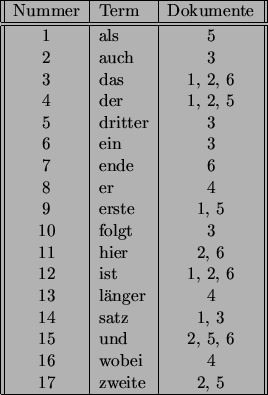
\includegraphics[scale=0.5]{../Abbildungen/index.png}
	\caption{Beispiel für einen invertierten Index \cite{index_Uni_Munich}}
\end{figure}

\subsection{Umsetzung eines invertierten Index}
Nachdem das Prinzip des invertierten Index klar ist, steht die Frage im Raum wie dieser umgesetzt werden kann.
Es liegt nahe als Datenstruktur einen Trie einzusetzen. Ein Trie ist ein spezieller Suchbaum, welcher besonders gut zum Suchen von Zeichenketten geeignet ist \cite{IR_Intro_Cambridge}.
\newline
Alternativ kann über den Einsatz einer Hasmap nachgedacht werden, jedoch führt dies zu folgendem Problem:
Angenommen eine vom Nutzer eingegebene Query ist nicht in der Hashmap vorhanden. Die Hash-Funktion wird einen Fehler werfen. Da in einer Hashmap Wörter, die ähnlich zueinander sind, nicht unbedingt benachbart gespeichert werden und keinerlei Information darüber bekannt ist, wo zur Query ähnliche Wörter gespeichert sind, kann im Falle, dass ein oder mehrere Wörter der Query nicht vorhanden sind, nicht mit geringem Aufwand nach ähnlichen Wörtern gesucht werden. Bei Tries besteht dieses Problem nicht \cite{IR_Intro_Cambridge}. 
\newline
Da in der Beispielimplementierung ein Trie als Datenstruktur zum Einsatz kommen wird, soll diese kurz vorgestellt werden.

\subsubsection{Tries}
Ein Trie wird auf der Basis einer Menge von Zeichenketten aufgebaut. Jede Zeichenkette, die gefunden werden muss, ist innerhalb des Tries repräsentiert.
\newline
Erreicht wird dies dadurch, dass ein Knoten jeweils ein Zeichen repräsentiert und eine Liste mit Verweisen auf die nächsten möglichen Knoten hält, basierend auf einem weiteren Zeichen.
Die folgende Abbildung zeigt einen Trie.

\begin{figure}[H]
	\centering
	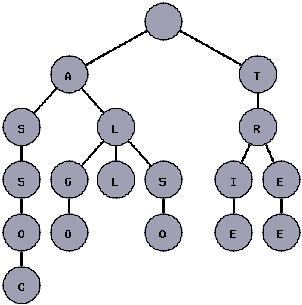
\includegraphics[scale=0.7]{../Abbildungen/trie.png}
	\caption{Beispiel eines Tries \cite{trie_Abb}}
\end{figure}

\newpage
Im Folgenden soll eine formale Definition eines Tries gegeben werden:
\newline
\begin{defi}
	Sei $\sum$ eine endliche Menge von Zeichen (Alphabet) und $\sum^{*}$ die Menge aller Wörter, die über $\sum$ gebildet werden können. Sei $S$ $\subseteq$ $\sum^{*}$. Dann ist $T = (V, E)$ ein Trie, wobei $V$ die Menge aller Knoten und $E$ die Menge aller Kanten ist. Darüber hinaus muss gelten:
	
	\begin{itemize}
		\item $\forall e \in E: e$ ist mit Zeichen aus $\sum$ beschriftet.
		\item $\forall v \in V:$ alle ausgehenden Kanten von $v$ sind unterschiedlich beschriftet mit einem Zeichen $z \in \sum$
		\item $\forall S_i \in S: \exists v \in V: S_i$ ist ein Präfix der Konkatenation der Beschriftungen des Pfades vom Wurzelknoten bis $v$.
		\item $\forall b \in V: \exists S_i \in S:$ Die Konkatenation der Beschriftungen von der Wurzel bis $b$ ergibt $S_i$, sofern $b$ ein Blatt des Tries ist.
	\end{itemize}
\end{defi}

Definition 27 ist aus \cite{Trie_wiki} entnommen.
\newline \newline
Das Suchen nach gespeicherten Wörtern gestaltet sich nun verhältnismäßig einfach: Um das Wort \glqq Tree\grqq im, in der Abbildung gezeigten, Trie zu finden, wird wie folgt vorgegangen.
\newline 
Stellt der User die Anfrage \glqq Tree\grqq wird diese Query nun Zeichen für Zeichen durchgegangen. Beginnend bei \glqq T\grqq wird im Wurzelknoten geprüft, ob es einen Verweis auf einen Knoten gibt, der ein \glqq T\grqq repräsentiert \cite{trie_Abb}. Existiert ein solcher Knoten, wird in diesem geprüft, ob es einen Knoten gibt, der das nächste Zeichen in der Query (das \glqq r\grqq) repräsentiert. Ist dies der Fall wird das Verfahren solange wiederholt bis die Query komplett eingelesen ist oder in der Query ein Zeichen steht, das durch keinen Knoten im Trie repräsentiert ist \cite{trie_Abb} \cite{Trie_Blog}.
\newline \newline
Ähnlich leicht funktioniert das Einfügen neuer Wörter in den Trie. Dazu wird - wie beim Suchen - das Wort, das eingefügt werden soll, so weit wie möglich nach dem oben beschriebenen Muster eingelesen und es wird zu den entsprechenden Knoten gesprungen \cite{trie_Abb} \cite{Trie_Blog}. Wird nun ein Zeichen eingelesen, das nicht durch einen Knoten repräsentiert ist, wird ein neuer Knoten erzeugt, welcher dieses Zeichen repräsentiert \cite{trie_Abb}. Alle nun noch einzulesenden Zeichen erhalten einen neuen Knoten, da der neu erzeugte Knoten natürlich nicht auf bereits vorhandene Knoten zeigen kann. Innerhalb dieses Knotens wird eine Liste angelegt, die Verweise auf weitere Knoten hält \cite{trie_Abb}. In dieser Liste wird ein Verweis auf den Knoten angelegt, der das nächste Zeichen des einzufügenden Wortes repräsentiert. Dieses Verfahren setzt sich solange fort, bis das neue Wort vollständig eingelesen ist.
\newline \newline
Das Löschen soll in diesem Rahmen nicht aufgezeigt werden, da dies weitaus komplexer sein kann als das Finden oder Einfügen von Einträgen.
\newline \newline
Ein Knoten, zu dem man mit dem Wort $S_i$ gelangt, muss außerdem eine Liste mit Verweisen auf alle Dokumente, in denen das Wort $S_i$ vorkommt, speichern. Gibt es keine Dokumente, in denen $S_i$ vorkommt, ist die Liste leer.

\section{Komprimierung des Index}
Bei großen Dokumentenmengen wächst die Größe des Index ebenfalls. Doch nicht nur die Größe des Index wächst, sondern auch die benötigte Zeit, um auf eine Query zu antworten \cite{IR_Intro_Cambridge}.
Die Index-Komprimierung adressiert genau dieses Problem. Über die Jahre der Forschung haben sich einige Komprimierungs-Techniken bewährt und sind bei den allermeisten aktuellen Suchmaschinen in Benutzung. \newline
Dieser Abschnitt soll das Thema Komprimierung erläutern, das Hauptaugenmerk liegt dabei auf der Komprimierungs-Technik, die in der Beispielimplementierung eingesetzt wird.

\section{TF-IDF Gewichtung}

\section{Retrieval}